\appendix
\renewcommand{\chaptername}{Appendix}
\chapter{Space convergence} \label{app:conv}
We report here some more convergence examples in addition to the Sin-Cos 
presented in Subsection~\ref{subsec:conv}.
%
\section{1D test}
We solve the equations~\eqref{eq:nssteadymass}--\eqref{eq:nssteadymom} over a 
one-dimensional unit domain $\Omega=(0,1)$, with the following source terms:
\begin{align}
	h &= 6x^2,\\
	f &= 12x^5 - 24\nu x - \frac{2}{\varrho} % con enableUnsymmetrizedGradient
\end{align}
so that, choosing $\varrho=1$, the analytical solution, depicted in 
Figure~\ref{fig:1dexact}, is given by
\begin{align}
\label{eq:uex1d}	u_\text{ex}(x) &= 2x^3\\
\label{eq:pex1d}	p_\text{ex}(x) &= 2-2x
\end{align}
Dirichlet boundary conditions for the velocity are applied on the whole 
boundary $\partial \Omega$ using the exact solution. The pressure is fixed at 
one point in order to match the exact solution \eqref{eq:pex1d}.
\begin{figure}
	\centering
	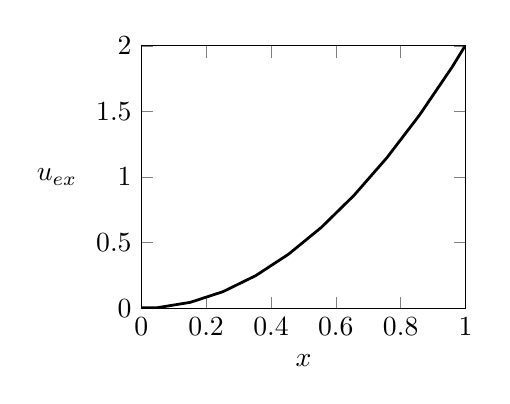
\begin{tikzpicture}
	\begin{axis}[width=0.47\textwidth, xlabel={$x$}, xmin=0, xmax=1, ymin=0, 
	ymax=2,	samples=100, ylabel={$u_\text{ex}$}, ylabel style={rotate=-90}]
	\addplot[color=black, mark=none, line width=1.0pt]{2*x*x};
	\end{axis}
	\end{tikzpicture}
%	\hskip 5pt
	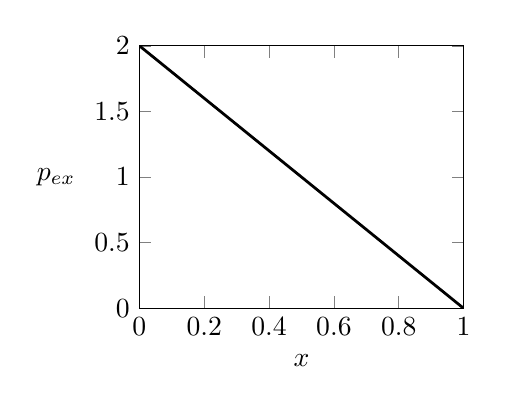
\begin{tikzpicture}
	\begin{axis}[width=0.47\textwidth, xlabel={$x$}, xmin=0, xmax=1, ymin=0, 
	ymax=2, samples=100, 
	ylabel={$p_\text{ex}$}, ylabel style={rotate=-90}]
	\addplot[color=black, mark=none, line width=1.0pt]{2*(1-x)};
	\end{axis}
	\end{tikzpicture}
	\caption[Exact solution of the 1D test]{Exact solution of the 1D test 
	\eqref{eq:uex1d}--\eqref{eq:pex1d}. On 
	the left the velocity field, on the right the pressure field.}
	\label{fig:1dexact}
\end{figure}

The problem is solved over a sequence of eight uniform grids, starting from 
4 cells and each time halving their size. Both the cases of $\nu=1$ 
and $\nu=\num{e-3}$ are considered, that correspond respectively to $Re=1$ and $Re=\num{e3}$. In Figure~\ref{fig:1d_err} the errors computed are reported 
depending on the number of cells, while in 
Tables~\ref{tab:1d_lre}--\ref{tab:1d_hre} we can compare directly the 
convergence orders for the different differencing schemes.
\begin{figure}
	\centering
	\subfloat[Upwind, $Re = 1$]{
		% This file was created by matlab2tikz.
%
\definecolor{mycolor1}{rgb}{0.00000,0.44700,0.74100}%
\definecolor{mycolor2}{rgb}{0.85000,0.32500,0.09800}%
%
\begin{tikzpicture}

\begin{axis}[%
width=0.951\figwidth,
height=0.75\figwidth,
at={(0\figwidth,0\figwidth)},
scale only axis,
xmode=log,
xmin=4,
xmax=1000,
xminorticks=true,
ymode=log,
ymin=1e-06,
ymax=1,
yminorticks=true,
axis background/.style={fill=white},
legend style={at={(0.03,0.03)}, anchor=south west, legend cell align=left, align=left, draw=white!15!black}
]
\addplot [color=mycolor1, mark=x, mark options={solid, mycolor1}]
  table[row sep=crcr]{%
4	0.214116295\\
8	0.195589151\\
16	0.132868874\\
32	0.0777359686\\
64	0.0420904681\\
128	0.0219065573\\
256	0.011175991\\
512	0.00564462389\\
};
\addlegendentry{$p$}

\addplot [color=mycolor2, mark=x, mark options={solid, mycolor2}]
  table[row sep=crcr]{%
4	0.0216704604\\
8	0.0117239406\\
16	0.00417857985\\
32	0.00124123493\\
64	0.000337955248\\
128	8.81570481e-05\\
256	2.25117773e-05\\
512	5.68790627e-06\\
};
\addlegendentry{$u$}

\addplot [color=white!70!black, forget plot]
  table[row sep=crcr]{%
4	0.00025\\
1000	1e-06\\
};
\addplot [color=white!70!black, forget plot]
  table[row sep=crcr]
	\subfloat[Upwind, $Re = \num{e3}$]{
		% This file was created by matlab2tikz.
%
\definecolor{mycolor1}{rgb}{0.00000,0.44700,0.74100}%
\definecolor{mycolor2}{rgb}{0.85000,0.32500,0.09800}%
%
\begin{tikzpicture}

\begin{axis}[%
width=0.951\figwidth,
height=0.75\figwidth,
at={(0\figwidth,0\figwidth)},
scale only axis,
xmode=log,
xmin=4,
xmax=1000,
xminorticks=true,
ymode=log,
ymin=0.001,
ymax=0.190700916,
yminorticks=true,
axis background/.style={fill=white},
legend style={at={(0.03,0.03)}, anchor=south west, legend cell align=left, align=left}
]
\addplot [color=mycolor1, mark=x, mark options={solid, mycolor1}]
  table[row sep=crcr]{%
4	0.0950934111\\
8	0.0956441228\\
16	0.0633456286\\
32	0.0359064412\\
64	0.0189587968\\
128	0.009733956\\
256	0.00507474159\\
512	0.00281243348\\
};
\addlegendentry{$p$}

\addplot [color=mycolor2, mark=x, mark options={solid, mycolor2}]
  table[row sep=crcr]{%
4	0.190700916\\
8	0.161981022\\
16	0.100050412\\
32	0.0542847205\\
64	0.0273944361\\
128	0.013011169\\
256	0.00574729458\\
512	0.00230500508\\
};
\addlegendentry{$u$}

\addplot [color=white!70!black, forget plot]
  table[row sep=crcr]{%
4	0.25\\
1000	0.001\\
};
\addplot [color=white!70!black, forget plot]
  table[row sep=crcr]\\
	\subfloat[Min-Mod, $Re = 1$]{
		% This file was created by matlab2tikz.
%
\definecolor{mycolor1}{rgb}{0.00000,0.44700,0.74100}%
\definecolor{mycolor2}{rgb}{0.85000,0.32500,0.09800}%
%
\begin{tikzpicture}

\begin{axis}[%
width=0.951\figwidth,
height=0.75\figwidth,
at={(0\figwidth,0\figwidth)},
scale only axis,
xmode=log,
xmin=4,
xmax=1000,
xminorticks=true,
ymode=log,
ymin=1e-07,
ymax=0.1,
yminorticks=true,
axis background/.style={fill=white},
legend style={at={(0.03,0.03)}, anchor=south west, legend cell align=left, align=left}
]
\addplot [color=mycolor1, mark=x, mark options={solid, mycolor1}]
  table[row sep=crcr]{%
4	0.0947400829\\
8	0.0579455977\\
16	0.0306653228\\
32	0.0155606681\\
64	0.00780733847\\
128	0.00390635907\\
256	0.0019533289\\
512	0.000976635645\\
};
\addlegendentry{$p$}

\addplot [color=mycolor2, mark=x, mark options={solid, mycolor2}]
  table[row sep=crcr]{%
4	0.00558067417\\
8	0.00185644832\\
16	0.000515125253\\
32	0.000134752887\\
64	3.44440641e-05\\
128	8.70859755e-06\\
256	2.18965445e-06\\
512	5.49000176e-07\\
};
\addlegendentry{$u$}

\addplot [color=white!70!black, forget plot]
  table[row sep=crcr]{%
4	2.5e-05\\
1000	1e-07\\
};
\addplot [color=white!70!black, forget plot]
  table[row sep=crcr]
	\subfloat[Min-Mod, $Re = \num{e3}$]{
		\input{../img/l2error_test_navierstokes_1d_mm_hre}}\\
	\subfloat[Van Leer, $Re = 1$]{
		% This file was created by matlab2tikz.
%
\definecolor{mycolor1}{rgb}{0.00000,0.44700,0.74100}%
\definecolor{mycolor2}{rgb}{0.85000,0.32500,0.09800}%
%
\begin{tikzpicture}

\begin{axis}[%
width=0.951\figwidth,
height=0.75\figwidth,
at={(0\figwidth,0\figwidth)},
scale only axis,
xmode=log,
xmin=4,
xmax=1000,
xminorticks=true,
ymode=log,
ymin=1e-07,
ymax=0.1,
yminorticks=true,
axis background/.style={fill=white},
legend style={at={(0.03,0.03)}, anchor=south west, legend cell align=left, align=left}
]
\addplot [color=mycolor1, mark=x, mark options={solid, mycolor1}]
  table[row sep=crcr]{%
4	0.058505198\\
8	0.0412346964\\
16	0.0251402529\\
32	0.0139748536\\
64	0.00738268213\\
128	0.00379649657\\
256	0.00192539001\\
512	0.000969591076\\
};
\addlegendentry{$p$}

\addplot [color=mycolor2, mark=x, mark options={solid, mycolor2}]
  table[row sep=crcr]{%
4	0.00804947871\\
8	0.0022466016\\
16	0.0005523443\\
32	0.000137569802\\
64	3.46360203e-05\\
128	8.7210858e-06\\
256	2.19045006e-06\\
512	5.49050369e-07\\
};
\addlegendentry{$u$}

\addplot [color=white!70!black, forget plot]
  table[row sep=crcr]{%
4	2.5e-05\\
1000	1e-07\\
};
\addplot [color=white!70!black, forget plot]
  table[row sep=crcr]
	\subfloat[Van Leer, $Re = \num{e3}$]{
		% This file was created by matlab2tikz.
%
\definecolor{mycolor1}{rgb}{0.00000,0.44700,0.74100}%
\definecolor{mycolor2}{rgb}{0.85000,0.32500,0.09800}%
%
\begin{tikzpicture}

\begin{axis}[%
width=0.951\figwidth,
height=0.75\figwidth,
at={(0\figwidth,0\figwidth)},
scale only axis,
xmode=log,
xmin=4,
xmax=1000,
xminorticks=true,
ymode=log,
ymin=1e-06,
ymax=0.1,
yminorticks=true,
axis background/.style={fill=white},
legend style={at={(0.03,0.03)}, anchor=south west, legend cell align=left, align=left, draw=white!15!black}
]
\addplot [color=mycolor1, mark=x, mark options={solid, mycolor1}]
  table[row sep=crcr]{%
4	0.0161844304\\
8	0.00984258579\\
16	0.00351641157\\
32	0.00101607975\\
64	0.000263342669\\
128	6.34168067e-05\\
256	1.44388667e-05\\
512	3.20413694e-06\\
};
\addlegendentry{$p$}

\addplot [color=mycolor2, mark=x, mark options={solid, mycolor2}]
  table[row sep=crcr]{%
4	0.0562254093\\
8	0.020321909\\
16	0.00583980329\\
32	0.0015266502\\
64	0.000376324406\\
128	8.75670102e-05\\
256	1.88988619e-05\\
512	3.69275832e-06\\
};
\addlegendentry{$u$}

\addplot [color=white!70!black, forget plot]
  table[row sep=crcr]{%
4	0.00025\\
1000	1e-06\\
};
\addplot [color=white!70!black, forget plot]
  table[row sep=crcr]
	\caption[$L^2$-errors for the 1D test]{$L^2$-errors for the 1D test 
	depending on the number of cells in the grid. The grey lines are the 
	reference lines for the first-order and second-order convergence.}
	\label{fig:1d_err}
\end{figure}
\begin{table}
	\centering
	\[
	\begin{array}{c|ccc}
	\toprule
	& \text{Upwind} & \text{Min-Mod} & \text{Van Leer} \\ 
	\midrule
	p & 0.985 & 1.000 & 0.990\\
	u & 1.985 & 1.996 & 1.996\\
	\bottomrule
	\end{array}
	\]
	\caption[Convergence orders with $Re = 1$ for the 1D test]{Convergence 
	orders with $Re = 1$ for the 1D test. They are computed considering the 
	last two refinements of the grid.}
	\label{tab:1d_lre}
	\[
	\begin{array}{c|ccc}
	\toprule
	& \text{Upwind} & \text{Min-Mod} & \text{Van Leer} \\ 
	\midrule
	p & 0.852 & 1.501 & 2.172\\
	u & 1.318 & 2.274 & 2.356\\
	\bottomrule
	\end{array}
	\]
	\caption[Convergence orders with $Re = \num{e3}$ for the 1D 
	test]{Convergence orders with $Re = \num{e3}$ for the 1D test. They 
	are computed considering the last two refinements of the grid.}
	\label{tab:1d_hre}
\end{table}

In this test, at $Re=1$, all the methods behave similarly, as we 
can see in Table~\ref{tab:1d_lre}, with the second-order convergence for the 
velocity also using the upwind method. Probably, in this one-dimensional 
configuration, the second-order diffusive term is dominating. From 
Table~\ref{tab:1d_hre} we observe instead that the TVD methods keep the second-order 
convergence for the velocity and increase the rate also for the pressure, while 
the upwind method decreases them. With the finest grid we observe from 
Figure~\ref{fig:1d_err} that with the TVD methods the errors are three orders of 
magnitude lower than with the upwind method.

%\FloatBarrier
%
\section{Kovasznay test}
We solve the equations~\eqref{eq:nssteadymass}--\eqref{eq:nssteadymom} over a 
two-dimensional domain $\Omega=(-0.5, 2) \times (-0.5,1.5)$, without any source 
term, so that, choosing $\varrho=1$, the analytical solution, depicted in 
Figure~\ref{fig:kovexact}, is given by
\begin{align}
\label{eq:uexkov} u_\text{ex}(x,y) &= 1-e^{\lambda x} \cos (2 \pi y)\\
v_\text{ex}(x,y) &= \frac{\lambda}{2\pi} e^{\lambda x} \sin (2\pi y)\\
\label{eq:pexkov}	p_\text{ex}(x,y) &= \frac{1}{2}(1 -e^{2\lambda x})\\
\lambda &= \frac{1}{2 \nu} - \sqrt{\frac{1}{4 \nu^2} + 4\pi^2},
\end{align}
as reported in \cite{test:kovasznay}.
Dirichlet boundary conditions for the velocity are applied on the whole 
boundary $\partial \Omega$ using the exact solution. The pressure is fixed at 
one point in order to match the exact solution \eqref{eq:pexkov}.
\begin{figure}
	\centering
	\subfloat{\includegraphics[width=0.5\textwidth]{kov_exact_v.png}}
	\subfloat{\includegraphics[width=0.5\textwidth]{kov_exact_p.png}}
	\caption[Exact solution of the Kovasznay test]{Exact solution of the 
	Kovasznay test \eqref{eq:uexkov}--\eqref{eq:pexkov}. On the left the 
	magnitude of the velocity field, on the 
	right the pressure field. The arrows are not scaled.}
	\label{fig:kovexact}
\end{figure}

The problem is solved over a sequence of seven uniform grids, starting from 
$\num{4x4}$ cells and each time halving their size. Both the cases of 
$\nu=\num{2.5e-2}$ and $\nu=\num{2.5e-4}$ are considered, that correspond respectively to 
$Re=80$ and $Re=\num{8e3}$. In Figure~\ref{fig:kov_err} the errors 
computed are reported depending on the number of cells, while in 
Tables~\ref{tab:kov_lre}--\ref{tab:kov_hre} we can compare directly the 
convergence orders for the different differencing schemes.
\begin{figure}
	\centering
	\subfloat[Upwind, $Re = 80$]{
		% This file was created by matlab2tikz.
%
\definecolor{mycolor1}{rgb}{0.00000,0.44700,0.74100}%
\definecolor{mycolor2}{rgb}{0.85000,0.32500,0.09800}%
\definecolor{mycolor3}{rgb}{0.92900,0.69400,0.12500}%
%
\begin{tikzpicture}

\begin{axis}[%
width=0.951\figwidth,
height=0.75\figwidth,
at={(0\figwidth,0\figwidth)},
scale only axis,
xmode=log,
xmin=4,
xmax=256,
xminorticks=true,
ymode=log,
ymin=0.000651880984,
ymax=1,
yminorticks=true,
axis background/.style={fill=white},
legend style={at={(0.03,0.03)}, anchor=south west, legend cell align=left, align=left, draw=white!15!black}
]
\addplot [color=mycolor1, mark=x, mark options={solid, mycolor1}]
  table[row sep=crcr]{%
4	0.463423878\\
8	0.143112573\\
16	0.0498339933\\
32	0.0274485113\\
64	0.0157273343\\
128	0.00905807802\\
256	0.00511952099\\
};
\addlegendentry{$p$}

\addplot [color=mycolor2, mark=x, mark options={solid, mycolor2}]
  table[row sep=crcr]{%
4	0.0365475504\\
8	0.0402359415\\
16	0.0284971904\\
32	0.016030142\\
64	0.00911637277\\
128	0.00494934791\\
256	0.00260057897\\
};
\addlegendentry{$u$}

\addplot [color=mycolor3, mark=x, mark options={solid, mycolor3}]
  table[row sep=crcr]{%
4	0.01620299\\
8	0.0203942699\\
16	0.00813891576\\
32	0.00425163801\\
64	0.00234145986\\
128	0.00125075128\\
256	0.000651880984\\
};
\addlegendentry{$v$}

\addplot [color=white!70!black, forget plot]
  table[row sep=crcr]{%
4	0.041720382976\\
256	0.000651880984\\
};
\addplot [color=white!70!black, forget plot]
  table[row sep=crcr]
	\subfloat[Upwind, $Re = \num{8e3}$]{
		% This file was created by matlab2tikz.
%
\definecolor{mycolor1}{rgb}{0.00000,0.44700,0.74100}%
\definecolor{mycolor2}{rgb}{0.85000,0.32500,0.09800}%
\definecolor{mycolor3}{rgb}{0.92900,0.69400,0.12500}%
%
\begin{tikzpicture}

\begin{axis}[%
width=0.951\figwidth,
height=0.75\figwidth,
at={(0\figwidth,0\figwidth)},
scale only axis,
xmode=log,
xmin=4,
xmax=256,
xminorticks=true,
ymode=log,
ymin=5.06127924e-05,
ymax=0.0108188379,
yminorticks=true,
axis background/.style={fill=white},
legend style={at={(0.03,0.03)}, anchor=south west, legend cell align=left, align=left}
]
\addplot [color=white!70!black, forget plot, line width=0.75pt]
  table[row sep=crcr]{%
4	0.0032392187136\\
256	5.06127924e-05\\
};
\addplot [color=white!70!black, forget plot, line width=0.75pt]
  table[row sep=crcr]{%
4	0.2073099976704\\
256	5.06127924e-05\\
};
\addplot [color=mycolor1, mark=x, mark options={solid, mycolor1}, line width=0.75pt]
  table[row sep=crcr]{%
4	0.0101205447\\
8	0.0108188379\\
16	0.00617459521\\
32	0.00142458715\\
64	0.00065817115\\
128	0.000326889512\\
256	0.000163405515\\
};
\addlegendentry{$p$}

\addplot [color=mycolor2, mark=x, mark options={solid, mycolor2}, line width=0.75pt]
  table[row sep=crcr]{%
4	0.000827330593\\
8	0.00859442106\\
16	0.00525853983\\
32	0.00227364257\\
64	0.00103524242\\
128	0.000497944856\\
256	0.000243793246\\
};
\addlegendentry{$u$}

\addplot [color=mycolor3, mark=x, mark options={solid, mycolor3}, line width=0.75pt]
  table[row sep=crcr]\\
	\subfloat[Min-Mod, $Re = 80$]{
		% This file was created by matlab2tikz.
%
\definecolor{mycolor1}{rgb}{0.00000,0.44700,0.74100}%
\definecolor{mycolor2}{rgb}{0.85000,0.32500,0.09800}%
\definecolor{mycolor3}{rgb}{0.92900,0.69400,0.12500}%
%
\begin{tikzpicture}

\begin{axis}[%
width=0.951\figwidth,
height=0.75\figwidth,
at={(0\figwidth,0\figwidth)},
scale only axis,
xmode=log,
xmin=4,
xmax=256,
xminorticks=true,
ymode=log,
ymin=1e-05,
ymax=1,
yminorticks=true,
axis background/.style={fill=white},
legend style={at={(0.03,0.03)}, anchor=south west, legend cell align=left, align=left}
]
\addplot [color=white!70!black, forget plot, line width=0.75pt]
  table[row sep=crcr]{%
4	0.00064\\
256	1e-05\\
};
\addplot [color=white!70!black, forget plot, line width=0.75pt]
  table[row sep=crcr]{%
4	0.04096\\
256	1e-05\\
};
\addplot [color=mycolor1, mark=x, mark options={solid, mycolor1}, line width=0.75pt]
  table[row sep=crcr]{%
4	0.465166938\\
8	0.211594301\\
16	0.136227298\\
32	0.104600388\\
64	0.0705134741\\
128	0.0412862288\\
256	0.0222713545\\
};
\addlegendentry{$p$}

\addplot [color=mycolor2, mark=x, mark options={solid, mycolor2}, line width=0.75pt]
  table[row sep=crcr]{%
4	0.0370158453\\
8	0.0494417118\\
16	0.0189924822\\
32	0.0070068795\\
64	0.0018286295\\
128	0.000384013264\\
256	7.098536e-05\\
};
\addlegendentry{$u$}

\addplot [color=mycolor3, mark=x, mark options={solid, mycolor3}, line width=0.75pt]
  table[row sep=crcr]
	\subfloat[Min-Mod, $Re = \num{8e3}$]{
		% This file was created by matlab2tikz.
%
\definecolor{mycolor1}{rgb}{0.00000,0.44700,0.74100}%
\definecolor{mycolor2}{rgb}{0.85000,0.32500,0.09800}%
\definecolor{mycolor3}{rgb}{0.92900,0.69400,0.12500}%
%
\begin{tikzpicture}

\begin{axis}[%
width=0.951\figwidth,
height=0.75\figwidth,
at={(0\figwidth,0\figwidth)},
scale only axis,
xmode=log,
xmin=4,
xmax=256,
xminorticks=true,
ymode=log,
ymin=1e-06,
ymax=0.010134474,
yminorticks=true,
axis background/.style={fill=white},
legend style={at={(0.03,0.03)}, anchor=south west, legend cell align=left, align=left}
]
\addplot [color=white!70!black, forget plot, line width=0.75pt]
  table[row sep=crcr]{%
4	6.4e-05\\
256	1e-06\\
};
\addplot [color=white!70!black, forget plot, line width=0.75pt]
  table[row sep=crcr]{%
4	0.004096\\
256	1e-06\\
};
\addplot [color=mycolor1, mark=x, mark options={solid, mycolor1}, line width=0.75pt]
  table[row sep=crcr]{%
4	0.010134474\\
8	0.00824868818\\
16	0.00116892786\\
32	0.000702043982\\
64	0.000420463449\\
128	0.000239681668\\
256	0.000127809753\\
};
\addlegendentry{$p$}

\addplot [color=mycolor2, mark=x, mark options={solid, mycolor2}, line width=0.75pt]
  table[row sep=crcr]{%
4	0.000766547494\\
8	0.00735792955\\
16	0.000706862636\\
32	0.00061606567\\
64	0.000254939342\\
128	9.30517021e-05\\
256	2.60788059e-05\\
};
\addlegendentry{$u$}

\addplot [color=mycolor3, mark=x, mark options={solid, mycolor3}, line width=0.75pt]
  table[row sep=crcr]\\
	\subfloat[Van Leer, $Re = 80$]{
		% This file was created by matlab2tikz.
%
\definecolor{mycolor1}{rgb}{0.00000,0.44700,0.74100}%
\definecolor{mycolor2}{rgb}{0.85000,0.32500,0.09800}%
\definecolor{mycolor3}{rgb}{0.92900,0.69400,0.12500}%
%
\begin{tikzpicture}

\begin{axis}[%
width=0.951\figwidth,
height=0.75\figwidth,
at={(0\figwidth,0\figwidth)},
scale only axis,
xmode=log,
xmin=4,
xmax=256,
xminorticks=true,
ymode=log,
ymin=1e-05,
ymax=1,
yminorticks=true,
axis background/.style={fill=white},
legend style={at={(0.03,0.03)}, anchor=south west, legend cell align=left, align=left, draw=white!15!black}
]
\addplot [color=mycolor1, mark=x, mark options={solid, mycolor1}]
  table[row sep=crcr]{%
4	0.465362151\\
8	0.217919739\\
16	0.139676226\\
32	0.108111944\\
64	0.0720073262\\
128	0.041719522\\
256	0.0223197113\\
};
\addlegendentry{$p$}

\addplot [color=mycolor2, mark=x, mark options={solid, mycolor2}]
  table[row sep=crcr]{%
4	0.0369687113\\
8	0.0508536301\\
16	0.0240504197\\
32	0.00891876699\\
64	0.00230043057\\
128	0.000492539951\\
256	9.46578832e-05\\
};
\addlegendentry{$u$}

\addplot [color=mycolor3, mark=x, mark options={solid, mycolor3}]
  table[row sep=crcr]{%
4	0.0170184173\\
8	0.0249081905\\
16	0.00786909699\\
32	0.00254735352\\
64	0.000629680162\\
128	0.000123018505\\
256	2.07816951e-05\\
};
\addlegendentry{$v$}

\addplot [color=white!70!black, forget plot]
  table[row sep=crcr]{%
4	0.00064\\
256	1e-05\\
};
\addplot [color=white!70!black, forget plot]
  table[row sep=crcr]
	\subfloat[Van Leer, $Re = \num{8e3}$]{
		% This file was created by matlab2tikz.
%
\definecolor{mycolor1}{rgb}{0.00000,0.44700,0.74100}%
\definecolor{mycolor2}{rgb}{0.85000,0.32500,0.09800}%
\definecolor{mycolor3}{rgb}{0.92900,0.69400,0.12500}%
%
\begin{tikzpicture}

\begin{axis}[%
width=0.951\figwidth,
height=0.75\figwidth,
at={(0\figwidth,0\figwidth)},
scale only axis,
xmode=log,
xmin=4,
xmax=256,
xminorticks=true,
ymode=log,
ymin=1e-06,
ymax=0.010132924,
yminorticks=true,
axis background/.style={fill=white},
legend style={at={(0.03,0.03)}, anchor=south west, legend cell align=left, align=left}
]
\addplot [color=mycolor1, mark=x, mark options={solid, mycolor1}]
  table[row sep=crcr]{%
4	0.010132924\\
8	0.00680316149\\
16	0.000677901356\\
32	0.000521130225\\
64	0.000372827168\\
128	0.000226965042\\
256	0.000124578854\\
};
\addlegendentry{$p$}

\addplot [color=mycolor2, mark=x, mark options={solid, mycolor2}]
  table[row sep=crcr]{%
4	0.000752792347\\
8	0.00792052753\\
16	0.000772150807\\
32	0.000461995506\\
64	0.000232426927\\
128	8.93024538e-05\\
256	2.52578072e-05\\
};
\addlegendentry{$u$}

\addplot [color=mycolor3, mark=x, mark options={solid, mycolor3}]
  table[row sep=crcr]{%
4	0.00040159829\\
8	0.00256437192\\
16	0.000197529591\\
32	0.000108825618\\
64	4.65481791e-05\\
128	1.4700347e-05\\
256	3.78297463e-06\\
};
\addlegendentry{$v$}

\addplot [color=white!70!black, forget plot]
  table[row sep=crcr]{%
4	6.4e-05\\
256	1e-06\\
};
\addplot [color=white!70!black, forget plot]
  table[row sep=crcr]
	\caption[$L^2$-errors for the Kovasznay test]{$L^2$-errors for the 
	Kovasznay test depending on the number of cells in the grid. The grey 
	lines are the reference lines for the first-order and second-order 
	convergence.}
	\label{fig:kov_err}
\end{figure}
\begin{table}
	\centering
	\[
	\begin{array}{c|ccc}
	\toprule
	& \text{Upwind} & \text{Min-Mod} & \text{Van Leer} \\ 
	\midrule
	p & 0.823 & 0.890 & 0.902\\
	u & 0.928 & 2.436 & 2.379\\
	v & 0.940 & 2.422 & 2.565\\
	\bottomrule
	\end{array}
	\]
	\caption[Convergence orders with $Re = 80$ for the Kovasznay 
	test]{Convergence orders with $Re = 80$ for the Kovasznay test. They 
	are computed considering the last two refinements of the grid.}
	\label{tab:kov_lre}
	\[
	\begin{array}{c|ccc}
	\toprule
	& \text{Upwind} & \text{Min-Mod} & \text{Van Leer} \\ 
	\midrule
	p & 1.000 & 0.907 & 0.865\\
	u & 1.030 & 1.835 & 1.822\\
	v & 0.997 & 1.960 & 1.958\\
	\bottomrule
	\end{array}
	\]
	\caption[Convergence orders with $Re = \num{8e3}$ for the Kovasznay 
	test]{Convergence orders with $Re = \num{8e3}$ for the Kovasznay 
	test. They are computed considering the last two refinements of the 
	grid.}
	\label{tab:kov_hre}
\end{table}

From Tables~\ref{tab:kov_lre} and \ref{tab:kov_hre}, we see that in this test 
the convergence results for $Re=80$ and $Re=\num{8e3}$ are very similar. With 
the upwind method the convergence orders are always 1, while with the TVD 
methods we obtain a second order, but only for the velocity. However, observing 
Figure~\ref{fig:kov_err}, the convergence orders for the TVD methods at 
$Re=\num{8e3}$ are increasing in the last four refinements.
%
%\section{Angeli test}
